% -*- latex -*-

\chapter{Fancy Array Storage}
\label{chap:Storage}

\index{array~handle|(}

Chapter~\ref{chap:ArrayHandle} introduces the \vtkmcont{ArrayHandle} class.
In it, we learned how an \textidentifier{ArrayHandle} manages the
memory allocation of an array, provides access to the data via array
portals, and supervises the movement of data between the control and
execution environments.

\index{array~handle!storage|(}
\index{storage|(}

In addition to these data management features, \textidentifier{ArrayHandle}
also provides a configurable \keyterm{storage} mechanism that allows you,
through efficient template configuration, to redefine how data are stored
and retrieved. The storage object provides an encapsulated interface around
the data so that any necessary strides, offsets, or other access patterns
may be handled internally. The relationship between array handles and their
storage object is shown in Figure~\ref{fig:ArrayHandleStorage}.

\begin{figure}[htb]
  \centering
  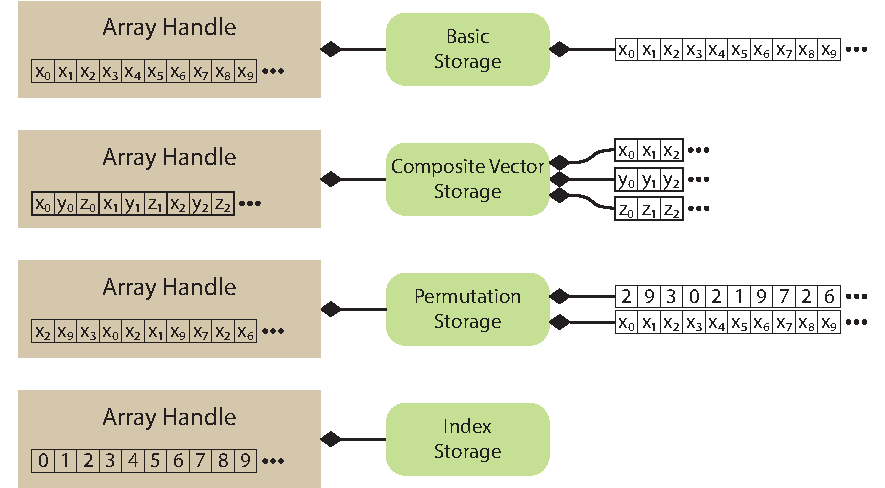
\includegraphics{images/ArrayHandleStorage}
  \caption{Array handles, storage objects, and the underlying data source.}
  \label{fig:ArrayHandleStorage}
\end{figure}

One interesting consequence of using a generic storage object to manage
data within an array handle is that the storage can be defined
functionally rather than point to data stored in physical memory. Thus,
implicit array handles are easily created by adapting to functional
``storage.'' For example, the point coordinates of a uniform rectilinear
grid are implicit based on the topological position of the point. Thus, the
point coordinates for uniform rectilinear grids can be implemented as an
implicit array with the same interface as explicit arrays (where
unstructured grid points would be stored). In this chapter we explore the
many ways you can manipulate the \textidentifier{ArrayHandle} storage.

\begin{didyouknow}
  VTK-m comes with many ``fancy'' array handles that can change the data in
  other arrays without modifying the memory or can generate data on the fly
  to behave like an array without actually using any memory. These fancy
  array handles are documented later in this chapter, and they can be very
  handy when developing with VTK-m.
\end{didyouknow}


\section{Basic Storage}

\index{array~handle!storage!default}
\index{storage!default}

As previously discussed in Chapter~\ref{chap:ArrayHandle},
\vtkmcont{ArrayHandle} takes two template arguments.
\begin{vtkmexample}{Declaration of the \protect\vtkmcont{ArrayHandle} templated class (again).}
template<
    typename T,
    typename StorageTag = VTKM_DEFAULT_STORAGE_TAG>
class ArrayHandle;
\end{vtkmexample}
The first argument is the only one required and has been demonstrated
multiple times before. The second (optional) argument specifies something
called a storage, which provides the interface between the generic
\vtkmcont{ArrayHandle} class and a specific storage mechanism in the
control environment.

In this and the following sections we describe this storage mechanism. A
default storage is specified in much the same way as a default device
adapter is defined (as described in Section~\ref{sec:DefaultDeviceAdapter}.
It is done by setting the \vtkmmacro{VTKM\_STORAGE} macro. This macro must
be set before including any VTK-m header files. Currently the only
practical storage provided by VTK-m is the basic storage, which simply
allocates a continuous section of memory of the given base type. This
storage can be explicitly specified by setting \vtkmmacro{VTKM\_STORAGE} to
\vtkmmacro{VTKM\_STORAGE\_BASIC} although the basic storage will also be
used as the default if no other storage is specified (which is typical).

The default storage can always be overridden by specifying an array
storage tag. The tag for the basic storage is located in the
\vtkmheader{vtkm/cont}{StorageBasic.h} header file and is named
\vtkmcont{StorageTagBasic}. Here is an example of specifying
the storage type when declaring an array handle.

\vtkmlisting{Specifying the storage type for an \textidentifier{ArrayHandle.}}{ArrayHandleStorageParameter.cxx}

VTK-m also defines a macro named \vtkmmacro{VTKM\_DEFAULT\_STORAGE\_TAG}
that can be used in place of an explicit storage tag to use the
default tag. This macro is used to create new templates that have template
parameters for storage that can use the default.


\index{array~handle!fancy|(}
\index{fancy~array~handle|(}

\section{Provided Fancy Arrays}
\label{sec:ProvidedFancyArrays}

The generic array handle and storage templating in VTK-m allows for
any type of operations to retrieve a particular value. Typically this is
used to convert an index to some location or locations in memory. However,
it is also possible to do many other operations. Arrays can be augmented on
the fly by mutating their indices or values. Or values could be computed
directly from the index so that no storage is required for the array at
all. This modified behavior for arrays is called ``fancy'' arrays.

VTK-m provides many of the fancy arrays, which we explore in this section.
Later Section~\ref{sec:ImplementingFancyArrays} describes many different
ways in which new fancy arrays can be implemented.

\subsection{Constant Arrays}
\label{sec:ConstantArrays}

\index{array~handle!constant|(}
\index{constant~array~handle|(}

A constant array is a fancy array handle that has the same value in all of
its entries. The constant array provides this array without actually using
any memory.

Specifying a constant array in VTK-m is straightforward. VTK-m has a class
named \vtkmcont{ArrayHandleConstant}. \textidentifier{ArrayHandleConstant}
is a templated class with a single template argument that is the type of
value for each element in the array. The constructor for
\textidentifier{ArrayHandleConstant} takes the value to provide by the
array and the number of values the array should present. The following
example is a simple demonstration of the constant array handle.

\vtkmlisting{Using \textidentifier{ArrayHandleConstant}.}{ArrayHandleConstant.cxx}

The \vtkmheader{vtkm/cont}{ArrayHandleConstant.h} header also contains the
templated convenience function \vtkmcont{make\_ArrayHandleConstant} that
takes a value and a size for the array. This function can sometimes be used
to avoid having to declare the full array type.

\vtkmlisting{Using \textidentifier{make\_ArrayHandleConstant}.}{MakeArrayHandleConstant.cxx}

\index{constant~array~handle|)}
\index{array~handle!constant|)}

\subsection{Counting Arrays}
\label{sec:CountingArrays}

\index{array~handle!counting|(}
\index{counting~array~handle|(}

A counting array is a fancy array handle that provides a sequence of
numbers. These fancy arrays can represent the data without actually using
any memory.

\index{array~handle!index|(}
\index{index~array~handle|(}

VTK-m provides two versions of a counting array. The first version is an
index array that provides a specialized but common form of a counting array
called an index array. An index array has values of type \vtkm{Id} that
start at 0 and count up by 1 (i.e. $0, 1, 2, 3,\ldots$). The index array
mirrors the array's index.

Specifying an index array in VTK-m is done with a class named
\vtkmcont{ArrayHandleIndex}. The constructor for
\textidentifier{ArrayHandleIndex} takes the size of the array to create.
The following example is a simple demonstration of the index array handle.

\vtkmlisting{Using \textidentifier{ArrayHandleIndex}.}{ArrayHandleIndex.cxx}

\index{index~array~handle|)}
\index{array~handle!index|)}

The \vtkmcont{ArrayHandleCounting} class provides a more general form of
counting. \textidentifier{ArrayHandleCounting} is a templated class with a
single template argument that is the type of value for each element in the
array. The constructor for \textidentifier{ArrayHandleCounting} takes three
arguments: the start value (used at index 0), the step from one value to
the next, and the length of the array. The following example is a simple
demonstration of the counting array handle.

\vtkmlisting{Using \textidentifier{ArrayHandleCounting}.}{ArrayHandleCountingBasic.cxx}

\begin{didyouknow}
  In addition to being simpler to declare,
  \textidentifier{ArrayHandleIndex} is slightly faster than
  \textidentifier{ArrayHandleCounting}. Thus, when applicable, you should
  prefer using \textidentifier{ArrayHandleIndex}.
\end{didyouknow}

The \vtkmheader{vtkm/cont}{ArrayHandleCounting.h} header also contains the
templated convenience function \vtkmcont{make\_ArrayHandleCounting} that
also takes the start value, step, and length as arguments. This function
can sometimes be used to avoid having to declare the full array type.

\vtkmlisting{Using \textidentifier{make\_ArrayHandleCounting}.}{MakeArrayHandleCountingBasic.cxx}

There are no fundamental limits on how \textidentifier{ArrayHandleCounting}
counts. For example, it is possible to count backwards.

\vtkmlisting{Counting backwards with \textidentifier{ArrayHandleCounting}.}{ArrayHandleCountingBackward.cxx}

It is also possible to use \textidentifier{ArrayHandleCounting} to make
sequences of \vtkm{Vec} values with piece-wise counting in each of the
components.

\vtkmlisting{Using \textidentifier{ArrayHandleCounting} with \protect\vtkm{Vec} objects.}{ArrayHandleCountingVec.cxx}

\index{counting~array~handle|)}
\index{array~handle!counting|)}

\subsection{Cast Arrays}
\label{sec:CastArrays}

\index{array~handle!cast|(}
\index{cast~array~handle|(}

A cast array is a fancy array that changes the type of the elements in an
array. The cast array provides this re-typed array without actually copying
or generating any data. Instead, casts are performed as the array is
accessed.

VTK-m has a class named \vtkmcont{ArrayHandleCast} to perform this implicit
casting. \textidentifier{ArrayHandleCast} is a templated class with two
template arguments. The first argument is the type to cast values to. The
second argument is the type of the original \textidentifier{ArrayHandle}.
The constructor to \textidentifier{ArrayHandleCast} takes the
\textidentifier{ArrayHandle} to modify by casting.

\vtkmlisting{Using \textidentifier{ArrayHandleCast}.}{ArrayHandleCast.cxx}

The \vtkmheader{vtkm/cont}{ArrayHandleCast.h} header also contains the
templated convenience function \vtkmcont{make\_ArrayHandleCast} that
constructs the cast array. The first argument is the original
\textidentifier{ArrayHandle} original array to cast. The optional second
argument is of the type to cast to (or you can optionally specify the
cast-to type as a template argument.

\vtkmlisting{Using \textidentifier{make\_ArrayHandleCast}.}{MakeArrayHandleCast.cxx}

\index{cast~array~handle|)}
\index{array~handle!cast|)}

\subsection{Permuted Arrays}
\label{sec:PermutedArrays}

\index{array~handle!permutation|(}
\index{permuted~array~handle|(}

A permutation array is a fancy array handle that reorders the elements in
an array. Elements in the array can be skipped over or replicated. The
permutation array provides this reordered array without actually coping any
data. Instead, indices are adjusted as the array is accessed.

Specifying a permutation array in VTK-m is straightforward. VTK-m has a
class named \vtkmcont{ArrayHandlePermutation} that takes two arrays: an
array of values and an array of indices that maps an index in the
permutation to an index of the original values. The index array is
specified first. The following example is a simple demonstration of the
permutation array handle.

\vtkmlisting{Using \textidentifier{ArrayHandlePermutation}.}{ArrayHandlePermutation.cxx}

The \vtkmheader{vtkm/cont}{ArrayHandlePermutation.h} header also contains the
templated convenience function \vtkmcont{make\_ArrayHandlePermutation} that
takes instances of the index and value array handles and returns a
permutation array. This function can sometimes be used to avoid having to
declare the full array type.

\vtkmlisting{Using \textidentifier{make\_ArrayHandlePermutation}.}{MakeArrayHandlePermutation.cxx}

\begin{commonerrors}
  When using an \textidentifier{ArrayHandlePermutation}, take care that all
  the provided indices in the index array point to valid locations in the
  values array. Bad indices can cause reading from or writing to invalid
  memory locations, which can be difficult to debug.
\end{commonerrors}

\index{permuted~array~handle|)}
\index{array~handle!permutation|)}

\subsection{Zipped Arrays}
\label{sec:ZippedArrays}

\index{array~handle!zip|(}
\index{zipped~array~handles|(}

A zip array is a fancy array handle that combines two arrays of the same
size to pair up the corresponding values. Each element in the zipped array
is a \vtkm{Pair} containing the values of the two respective arrays. These
pairs are not stored in their own memory space. Rather, the pairs are
generated as the array is used.

Specifying a zipped array in VTK-m is straightforward. VTK-m has a class
named \vtkmcont{ArrayHandleZip} that takes the two arrays providing values
for the first and second entries in the pairs. The following example is a
simple demonstration of creating a zip array handle.

\vtkmlisting{Using \textidentifier{ArrayHandleZip}.}{ArrayHandleZip.cxx}

The \vtkmheader{vtkm/cont}{ArrayHandleZip.h} header also contains the
templated convenience function \vtkmcont{make\_ArrayHandleZip} that takes
instances of the two array handles and returns a zip array. This function
can sometimes be used to avoid having to declare the full array type.

\vtkmlisting{Using \textidentifier{make\_ArrayHandleZip}.}{MakeArrayHandleZip.cxx}

\index{zipped~array~handles|)}
\index{array~handle!zip|)}

\subsection{Coordinate System Arrays}
\label{sec:CoordinateSystemArrays}

Many of the data structures we use in VTK-m are described in a 3D
coordinate system. Although, as we will see in Chapter~\ref{chap:DataSets},
we can use any \textidentifier{ArrayHandle} to store point coordinates,
including a raw array of 3D vectors, there are some common patterns for
point coordinates that we can use specialized arrays to better represent
the data.

\index{array~handle!uniform~point~coordinates|(}
\index{uniform~point~coordinates~array~handle|(}

There are two fancy array handles that each handle a special form of
coordinate system. The first such array handle is
\vtkmcont{ArrayHandleUniformPointCoordinates}, which represents a uniform
sampling of space. The constructor for
\textidentifier{ArrayHandleUniformPointCoordinates} takes three arguments.
The first argument is a \vtkm{Id3} that specifies the number of samples in
the $x$, $y$, and $z$ directions. The second argument, which is optional,
specifies the origin (the location of the first point at the lower left
corner). If not specified, the origin is set to $[0,0,0]$. The third
argument, which is also optional, specifies the distance between samples in
the $x$, $y$, and $z$ directions. If not specified, the spacing is set to
$1$ in each direction.

\vtkmlisting{Using \textidentifier{ArrayHandleUniformPointCoordinates}.}{ArrayHandleUniformPointCoordinates.cxx}

\index{uniform~point~coordinates~array~handle|)}
\index{array~handle!uniform~point~coordinates|)}

\index{array~handle!Cartesian~product|(}
\index{array~handle!rectilinear~point~coordinates|(}
\index{Cartesian~product~array~handle|(}
\index{rectilinear~point~coordinates~array~handle|(}

The second fancy array handle for special coordinate systems is
\vtkmcont{ArrayHandleCartesianProduct}, which represents a rectilinear
sampling of space where the samples are axis aligned but have variable
spacing. Sets of coordinates of this type are most efficiently represented
by having a separate array for each component of the axis, and then for
each $[i,j,k]$ index of the array take the value for each component from
each array using the respective index. This is equivalent to performing a
Cartesian product on the arrays.

\textidentifier{ArrayHandleCartesianProduct} is a templated class. It has
three template parameters, which are the types of the arrays used for the
$x$, $y$, and $z$ axes. The constructor for
\textidentifier{ArrayHandleCartesianProduct} takes the three arrays.

\vtkmlisting{Using a \textidentifier{ArrayHandleCartesianProduct}.}{ArrayHandleCartesianProduct.cxx}

The \vtkmheader{vtkm/cont/ArrayHandleCartesianProduct.h} header also
contains the templated convenience function
\vtkmcont{make\_ArrayHandleCartesianProduct} that takes the three axis
arrays and returns an array of the Cartesian product. This function can
sometimes be used to avoid having to declare the full array type.

\vtkmlisting{Using \textidentifier{make\_ArrayHandleCartesianProduct}.}{MakeArrayHandleCartesianProduct.cxx}

\index{rectilinear~point~coordinates~array~handle|)}
\index{Cartesian~product~array~handle|)}
\index{array~handle!rectilinear~point~coordinates|)}
\index{array~handle!Cartesian~product|)}

\begin{didyouknow}
  These specialized arrays for coordinate systems greatly reduce the code
  duplication in VTK-m. Most scientific visualization systems need separate
  implementations of algorithms for uniform, rectilinear, and unstructured
  grids. But in VTK-m an algorithm can be written once and then applied to
  all these different grid structures by using these specialized array
  handles and letting the compiler's templates optimize the code.
\end{didyouknow}

\subsection{Composite Vector Arrays}
\label{sec:CompositeVectorArrays}

\index{array~handle!composite~vector~arrays|(}
\index{composite~vector~arrays~array~handle|(}

A composite vector array is a fancy array handle that combines two to four
arrays of the same size and value type and combines their corresponding
values to form a \vtkm{Vec}. A composite vector array is similar in nature
to a zipped array (described in Section~\ref{sec:ZippedArrays}) except that
values are combined into \vtkm{Vec}s instead of \vtkm{Pair}s. The created
\vtkm{Vec}s are not stored in their own memory space. Rather, the pairs are
generated as the array is used.

A composite vector array can be created using the
\vtkmcont{ArrayHandleCompositeVector} class. This class has a single
template argument that is a ``signature'' for the arrays to be combined.
These signatures can be tricky to prototype, so
\vtkmheader{vtkm/cont/ArrayHandleCompositeVector.h} header also contains a
helper struct named \vtkmcont{ArrayHandleCompositeVectorType} to define the
type. \textidentifier{ArrayHandleCompositeVectorType} takes a variable
number of \textidentifier{ArrayHandle} types that compose the vector.
\textidentifier{ArrayHandleCompositeVectorType} has an internal type named
\textcode{type} that is the appropriately defined
\textidentifier{ArrayHandleCompositeVector}.

The constructor for \textidentifier{ArrayHandleCompositeVector} takes
instances of the array handles to combine along with the component from
each array to use. If the array handles being combined contain scalar data,
then the appropriate component to use is 0.

\vtkmlisting{Using \textidentifier{ArrayHandleCompositeVector}.}{ArrayHandleCompositeVectorBasic.cxx}

The \vtkmheader{vtkm/cont}{ArrayHandleCompositeVector.h} header also
contains the templated convenience function
\vtkmcont{make\_ArrayHandleCompositeVector} which takes two to four array
handles and returns an \textidentifier{ArrayHandleCompositeVector}. This
function can sometimes be used to avoid having to declare the full array
type.

\vtkmlisting{Using \textidentifier{make\_ArrayHandleCompositeVector}.}{MakeArrayHandleCompositeVector.cxx}

\textidentifier{ArrayHandleCompositeVector} is often used to combine scalar
arrays into vector arrays, but it can also be used to pull components out
of other vector arrays. The following example uses this feature to convert
an array of 2D $x,y$ coordinates and an array of elevations to 3D $x,y,z$
coordinates.

\vtkmlisting{Combining vector components with \textidentifier{ArrayHandleCompositeVector}.}{ArrayHandleCompositeVectorComponents.cxx}

\index{composite~vector~arrays~array~handle|)}
\index{array~handle!composite~vector~arrays|)}

\subsection{Grouped Vector Arrays}
\label{sec:GroupedVectorArrays}

\index{array~handle!group~vector|(}
\index{group~vector~array~handle|(}

\fix{Write this}

\index{group~vector~array~handle|)}
\index{array~handle!group~vector|)}


\section{Implementing Fancy Arrays}
\label{sec:ImplementingFancyArrays}

Although the behavior of fancy arrays might seem complicated, they are
actually straightforward to implement. VTK-m provides several mechanisms to
implement fancy arrays.

\subsection{Implicit Array Handles}

\index{array~handle!implicit|(}
\index{storage!implicit|(}
\index{implicit~storage|(}
\index{implicit~array~handle|(}
\index{functional~array|(}

The generic array handle and storage templating in VTK-m allows for
any type of operations to retrieve a particular value. Typically this is
used to convert an index to some location or locations in memory. However,
it is also possible to compute a value directly from an index rather than
look up some value in memory. Such an array is completely functional and
requires no storage in memory at all. Such a functional array is called an
\keyterm{implicit array handle}. Implicit arrays are an example of
\keyterm{fancy array handles}, which are array handles that behave like
regular arrays but do special processing under the covers to provide
values.

Specifying a functional or implicit array in VTK-m is straightforward.
VTK-m has a special class named \vtkmcont{ArrayHandleImplicit} that makes
an implicit array containing values generated by a user-specified
\keyterm{functor}. \index{functor} A functor is simply a C++ class or
struct that contains an overloaded parenthesis operator so that it can be
used syntactically like a function.

To demonstrate the use of \textidentifier{ArrayHandleImplicit}, let us say
we want an array of even numbers. The array has the values
$[0,2,4,6,\ldots]$ (double the index) up to some given size. Although we
could easily create this array in memory, we can save space and possibly
time by computing these values on demand.

\begin{didyouknow}
  VTK-m already comes with an implicit array handle named
  \vtkmcont{ArrayHandleCounting} that can make implicit even numbers as
  well as other more general counts. So in practice you would not have to
  create a special implicit array, but we are doing so here for
  demonstrative purposes.
\end{didyouknow}

The first step to using \textidentifier{ArrayHandleImplicit} is to declare
a functor. The functor's parenthesis operator should accept a single
argument of type \vtkm{Id} and return a value appropriate for that index.
The parenthesis operator should also be declared \textcode{const} because
it is not allowed to change the class' state.

\vtkmlisting{Functor that doubles an index.}{ImplicitArrayFunctor.cxx}

Once the functor is defined, an implicit array can be declared using the
templated \vtkmcont{ArrayHandleImplicit} class. The first template argument
is the type of the array's values (which should match the return value for
the functor), and the second template argument is the functor type.

\vtkmlisting{Declaring a \textidentifier{ArrayHandleImplicit}.}{DeclareImplicitArray.cxx}

For convenience, \vtkmheader{vtkm/cont}{ArrayHandleImplicit.h} also
declares the \vtkmcont{make\_ArrayHandleImplicit} function. This function
takes a functor and the size of the array and returns the implicit array.
When using this function, you also have to declare the first template
argument, which is the array's value type, since this type does not appear
in any of the arguments.

\vtkmlisting{Using \textidentifier{make\_ArrayHandleImplicit}.}{MakeArrayHandleImplicit.cxx}

\index{array~handle!subclassing}

If the implicit array you are creating tends to be generally useful and is
something you use multiple times, it might be worthwhile to make a
convenience subclass of \vtkmcont{ArrayHandleImplicit} for your array.

\vtkmlisting[ex:ImplicitArrayHandleSubclass]{Custom implicit array handle for even numbers.}{ImplicitArrayHandle2.cxx}

Subclasses of \textidentifier{ArrayHandle} provide constructors that
establish the state of the array handle. All array handle subclasses must
also use either the \vtkmmacro{VTKM\_ARRAY\_HANDLE\_SUBCLASS} macro or the
\vtkmmacro{VTKM\_ARRAY\_HANDLE\_SUBCLASS\_NT} macro. Both of these macros
define the typedefs \textcode{Superclass}, \textcode{ValueType}, and
\textcode{StorageTag} as well as a set of constructors and operators
expected of all \textidentifier{ArrayHandle} classes. The difference
between these two macros is that \vtkmmacro{VTKM\_ARRAY\_HANDLE\_SUBCLASS}
is used in templated classes whereas
\vtkmmacro{VTKM\_ARRAY\_HANDLE\_SUBCLASS\_NT} is used in non-templated
classes.

The \textidentifier{ArrayHandle} subclass in
Example~\ref{ex:ImplicitArrayHandleSubclass} is not templated, so it uses
the \vtkmmacro{VTKM\_ARRAY\_HANDLE\_SUBCLASS\_NT} macro. (The other macro
is described in Section~\ref{sec:VTKM_ARRAY_HANDLE_SUBCLASS} on
page~\pageref{sec:VTKM_ARRAY_HANDLE_SUBCLASS}). This macro takes two
parameters. The first parameter is the name of the subclass where the macro
is defined and the second parameter is the immediate superclass including
the full template specification. The second parameter of the macro must be
enclosed in parentheses so that the C pre-processor correctly handles
commas in the template specification.

\index{functional~array|)}
\index{implicit~array~handle|)}
\index{implicit~storage|)}
\index{storage!implicit|)}
\index{array~handle!implicit|)}

\subsection{Transformed Arrays}
\label{sec:TransformedArrays}

\index{array~handle!transform|(}
\index{transformed~array|(}

Another type of fancy array handle is the transformed array. A transformed
array takes another array and applies a function to all of the elements to
produce a new array. A transformed array behaves much like a map operation
except that a map operation writes its values to a new memory location
whereas the transformed array handle produces its values on demand so that
no additional storage is required.

Specifying a transformed array in VTK-m is straightforward. VTK-m has a
special class named \vtkmcont{ArrayHandleTransform} that takes an array
handle and a functor and provides an interface to a new array comprising
values of the first array applied to the functor.

To demonstrate the use of \textidentifier{ArrayHandleTransform}, let us say
that we want to scale and bias all of the values in a target array. That
is, each value in the target array is going to be multiplied by a given
scale and then offset by adding a bias value. (The scale and bias are
uniform across all entries.) We could, of course, easily create a worklet
to apply this scale and bias to each entry in the target array and save the
result in a new array, but we can save space and possibly time by computing
these values on demand.

The first step to using \textidentifier{ArrayHandleTransform} is to declare
a functor. The functor's parenthesis operator should accept a single
argument of the type of the target array and return the transformed value.
For more generally applicable transform functors, it is often useful to
make the parenthesis operator a template. The parenthesis operator should
also be declared \textcode{const} because it is not allowed to change the
class' state.

\vtkmlisting{Functor to scale and bias a value.}{TransformArrayFunctor.cxx}

Once the functor is defined, a transformed array can be declared using the
templated \vtkmcont{ArrayHandleTransform} class. The first template
argument is the type of the array's values (which should match the return
value for the functor). The second template argument is the type of array
being transformed. The third and final template argument is the type of
functor used for the transformation.

That said, it is generally easier to use the
\vtkmcont{make\_ArrayHandleTransform} convenience function. This function
takes an array and a functor and returns a transformed array. When using
this function, you also have to declare the first template argument, which
is the transformed array's value type, since this type does not appear in
any of the arguments.

\vtkmlisting{Using \textidentifier{make\_ArrayHandleTransform}.}{MakeArrayHandleTransform.cxx}

If the transformed array you are creating tends to be generally useful and
is something you use multiple times, it might be worthwhile to make a
convenience subclass of \vtkmcont{ArrayHandleTransform} or convenience
\textcode{make\_ArrayHandle*} function for your array.

\vtkmlisting[ex:TransformArrayHandleSubclass]{Custom transform array handle for scale and bias.}{TransformArrayHandle.cxx}

\label{sec:VTKM_ARRAY_HANDLE_SUBCLASS}

Subclasses of \textidentifier{ArrayHandle} provide constructors that
establish the state of the array handle. All array handle subclasses must
also use either the \vtkmmacro{VTKM\_ARRAY\_HANDLE\_SUBCLASS} macro or the
\vtkmmacro{VTKM\_ARRAY\_HANDLE\_SUBCLASS\_NT} macro. Both of these macros
define the typedefs \textcode{Superclass}, \textcode{ValueType}, and
\textcode{StorageTag} as well as a set of constructors and operators
expected of all \textidentifier{ArrayHandle} classes. The difference
between these two macros is that \vtkmmacro{VTKM\_ARRAY\_HANDLE\_SUBCLASS}
is used in templated classes whereas
\vtkmmacro{VTKM\_ARRAY\_HANDLE\_SUBCLASS\_NT} is used in non-templated
classes.

The \textidentifier{ArrayHandle} subclass in
Example~\ref{ex:TransformArrayHandleSubclass} is templated, so it uses the
\vtkmmacro{VTKM\_ARRAY\_HANDLE\_SUBCLASS} macro. (The other macro is
described in Section~\ref{sec:VTKM_ARRAY_HANDLE_SUBCLASS_NT} on
page~\pageref{sec:VTKM_ARRAY_HANDLE_SUBCLASS_NT}). This macro takes three
parameters. The first parameter is the name of the subclass where the macro
is defined, the second parameter is the type of the subclass including the
full template specification, and the third parameter is the immediate
superclass including the full template specification. The second and third
parameters of the macro must be enclosed in parentheses so that the C
pre-processor correctly handles commas in the template specification.

\index{transformed~array|)}
\index{array~handle!transform|)}


\subsection{Derived Storage}
\label{sec:DerivedStorage}

\index{array~handle!derived|(}
\index{storage!derived|(}
\index{derived~storage|(}

A \keyterm{derived storage} is a type of fancy array that takes one or more
other arrays and changes their behavior in some way. A transformed array
(Section~\ref{sec:TransformedArrays}) is a specific type of derived array
with a simple mapping. In this section we will demonstrate the steps
required to create a more general derived storage. When applicable, it is
much easier to create a derived array as a transformed array or using the
other fancy arrays than to create your own derived storage. However, if
these pre-existing fancy arrays do not work work, for example if your
derivation uses multiple arrays or requires general lookups, you can do so
by creating your own derived storage. For the purposes of the example in
this section, let us say we want 2 array handles to behave as one array
with the contents concatenated together. We could of course actually copy
the data, but we can also do it in place.

The first step to creating a derived storage is to build an array portal
that will take portals from arrays being derived. The portal must work in
both the control and execution environment (or have a separate version for
control and execution).

\vtkmlisting[ex:DerivedArrayPortal]{Derived array portal for concatenated arrays.}{DerivedArrayPortal.cxx}

Like in an adapter storage, the next step in creating a derived storage
is to define a tag for the adapter. We shall call ours
\textcode{StorageTagConcatenate} and it will be templated on
the two array handle types that we are deriving. Then, we need to create a
specialization of the templated \vtkmcontinternal{Storage}
class. The implementation for a \textidentifier{Storage} for
a derived storage is usually trivial compared to an adapter storage
because the majority of the work is deferred to the derived arrays.

\vtkmlisting[ex:DerivedArrayStorage]{\textidentifier{Storage} for derived container of concatenated arrays.}{DerivedArrayStorage.cxx}

One of the responsibilities of an array handle is to copy data between the
control and execution environments. The default behavior is to request the
device adapter to copy data items from one environment to another. This
might involve transferring data between a host and device. For an array of
data resting in memory, this is necessary. However, implicit storage
(described in the previous section) overrides this behavior to pass nothing
but the functional array portal. Likewise, it is undesirable to do a raw
transfer of data with derived storage. The underlying arrays being
derived may be used in other contexts, and it would be good to share the
data wherever possible. It is also sometimes more efficient to copy data
independently from the arrays being derived than from the derived storage
itself.

\index{array~transfer|(}

The mechanism that controls how a particular storage gets
transferred to and from the execution environment is encapsulated in the
templated \vtkmcontinternal{ArrayTransfer} class. By creating a
specialization of \vtkmcontinternal{ArrayTransfer}, we can modify the
transfer behavior to instead transfer the arrays being derived and use the
respective copies in the control and execution environments.

\vtkmcontinternal{ArrayTransfer} has three template arguments: the base type
of the array, the storage tag, and the device adapter tag.

\vtkmlisting[ex:ArrayTransferPrototype]{Prototype for \protect\vtkmcontinternal{ArrayTransfer}.}{ArrayTransferPrototype.cxx}

All \vtkmcontinternal{ArrayTransfer} implementations must have a
constructor method that accepts a pointer to a \vtkmcontinternal{Storage}
object templated to the same base type and storage tag as the
\textidentifier{ArrayTransfer} object. Assuming that an
\textidentifier{ArrayHandle} is templated using the parameters in
Example~\ref{ex:ArrayTransferPrototype}, the prototype for the constructor
must be equivalent to the following.
\begin{vtkmexample}{Prototype for \textidentifier{ArrayTransfer} constructor.}
ArrayTransfer(vtkm::cont::internal::Storage<T, StorageTag> *storage);
\end{vtkmexample}
Typically the constructor either saves the \textidentifier{Storage} pointer
or other relevant objects from the \textidentifier{Storage} for later use in
the methods.

In addition to this non-default constructor, the
\vtkmcontinternal{ArrayTransfer} specialization must define the following
items.
\begin{description}
\item[\textcode{ValueType}] A \textcode{typedef} of the type for each item
  in the array. This is the same type as the first template argument.
\item[\textcode{PortalControl}] The type of an array portal that is used to
  access the underlying data in the control environment.
\item[\textcode{PortalConstControl}] A read-only (const) version of
  \textcode{PortalControl}.
\item[\textcode{PortalExecution}] The type of an array portal that is used
  to access the underlying data in the execution environment.
\item[\textcode{PortalConstExecution}] A read-only (const) version of
  \textcode{PortalExecution}.
\item[\textcode{GetNumberOfValues}] A method that returns the number of
  values currently allocated in the execution environment. The results may
  be undefined if none of the load or allocate methods have yet been
  called.
\item[\textcode{PrepareForInput}] A method responsible for transferring
  data from the control to the execution for input.
  \textcode{PrepareForInput} has one Boolean argument that controls whether
  this transfer should actually take place. When true, data from the
  \textidentifier{Storage} object given in the constructor should be
  transferred to the execution environment; otherwise the data should not
  be copied. An \textidentifier{ArrayTransfer} for a derived array
  typically ignores this parameter since the arrays being derived manages
  this transfer already. Regardless of the Boolean flag, a
  \textcode{PortalConstExecution} is returned.
\item[\textcode{PrepareForInPlace}] A method that behaves just like
  \textcode{PrepareForInput} except that the data in the execution
  environment is used for both reading and writing so the method returns a
  \textidentifier{PortalExecution}. If the array is considered read-only,
  which is common for derived arrays, then this method should throw a
  \vtkmcont{ErrorControlBadValue}.
\item[\textcode{PrepareForOutput}] A method that takes a size (in a
  \vtkm{Id}) and allocates an array in the execution environment of the
  specified size. The initial memory can be uninitialized. The method
  returns a \textcode{PortalExecution} for the allocated data. If the array
  is considered read-only, which is common for derived arrays, then this
  method should throw a \vtkmcont{ErrorControlBadValue}.
\item[\textcode{RetrieveOutputData}] This method takes an array storage
  pointer (which is the same as that passed to the constructor, but
  provided for convenience), allocates memory in the control environment,
  and copies data from the execution environment into it. If the derived
  array is considered read-only and both \textcode{PrepareForInPlace} and
  \textcode{PrepareForOutput} throw exceptions, then this method should
  never be called. If it is, then that is probably a bug in
  \textidentifier{ArrayHandle}, and it is OK to throw
  \vtkmcont{ErrorControlInternal}.
\item[\textcode{Shrink}] A method that adjusts the size of the array in the
  execution environment to something that is a smaller size. All the data
  up to the new length must remain valid. Typically, no memory is actually
  reallocated. Instead, a different end is marked. If the derived array is
  considered read-only, then this method should throw a
  \vtkmcont{ErrorControlBadValue}.
\item[\textcode{ReleaseResources}] A method that frees any resources
  (typically memory) in the execution environment.
\end{description}

Continuing our example derived storage that concatenates two arrays
started in Examples \ref{ex:DerivedArrayPortal} and
\ref{ex:DerivedArrayStorage}, the following provides an
\textidentifier{ArrayTransfer} appropriate for the derived storage.

\vtkmlisting[ex:DerivedArrayTransfer]{\textidentifier{ArrayTransfer} for derived storage of concatenated arrays.}{DerivedArrayTransfer.cxx}

\index{array~transfer|)}

\index{array~handle!subclassing}

The final step to make a derived storage is to create a mechanism to
construct an \textidentifier{ArrayHandle} with a storage derived from the
desired arrays. This can be done by creating a trivial subclass of
\vtkmcont{ArrayHandle} that simply constructs the array handle to the state
of an existing storage. It uses a protected constructor of
\vtkmcont{ArrayHandle} that accepts a constructed storage.

\vtkmlisting[ex:DerivedArrayHandle]{\textidentifier{ArrayHandle} for derived storage of concatenated arrays.}{DerivedArrayHandle.cxx}

Subclasses of \textidentifier{ArrayHandle} provide constructors that
establish the state of the array handle. All array handle subclasses must
also use either the \vtkmmacro{VTKM\_ARRAY\_HANDLE\_SUBCLASS} macro or the
\vtkmmacro{VTKM\_ARRAY\_HANDLE\_SUBCLASS\_NT} macro. Both of these macros
define the typedefs \textcode{Superclass}, \textcode{ValueType}, and
\textcode{StorageTag} as well as a set of constructors and operators
expected of all \textidentifier{ArrayHandle} classes. The difference
between these two macros is that \vtkmmacro{VTKM\_ARRAY\_HANDLE\_SUBCLASS}
is used in templated classes whereas
\vtkmmacro{VTKM\_ARRAY\_HANDLE\_SUBCLASS\_NT} is used in non-templated
classes.

The \textidentifier{ArrayHandle} subclass in
Example~\ref{ex:DerivedArrayHandle} is templated, so it uses the
\vtkmmacro{VTKM\_ARRAY\_HANDLE\_SUBCLASS} macro. (The other macro is
described in Section~\ref{sec:VTKM_ARRAY_HANDLE_SUBCLASS_NT} on
page~\pageref{sec:VTKM_ARRAY_HANDLE_SUBCLASS_NT}). This macro takes three
parameters. The first parameter is the name of the subclass where the macro
is defined, the second parameter is the type of the subclass including the
full template specification, and the third parameter is the immediate
superclass including the full template specification. The second and third
parameters of the macro must be enclosed in parentheses so that the C
pre-processor correctly handles commas in the template specification.

\vtkmcont{ArrayHandleCompositeVector} is an example of a derived array
handle provided by VTK-m. It references some fixed number of other arrays,
pulls a specified component out of each, and produces a new component that
is a tuple of these retrieved components.

\index{derived~storage|)}
\index{storage!derived|)}
\index{array~handle!derived|)}

\index{array~handle!fancy|)}
\index{fancy~array~handle|)}



\section{Adapting Data Structures}
\label{sec:ArrayHandle:Adapting}

\index{array~handle!adapting|(}
\index{storage!adapting|(}

The intention of the storage parameter for \vtkmcont{ArrayHandle} is to
implement the strategy design pattern to enable VTK-m to interface directly
with the data of any third party code source. VTK-m is designed to work
with data originating in other libraries or applications. By creating a new
type of storage, VTK-m can be entirely adapted to new kinds of data
structures.

\begin{commonerrors}
  Keep in mind that memory layout used can have an effect on the running
  time of algorithms in VTK-m. Different data layouts and memory access can
  change cache performance and introduce memory affinity problems. The
  example code given in this section will likely have poorer cache
  performance than the basic storage provided by VTK-m. However, that might
  be an acceptable penalty to avoid data copies.
\end{commonerrors}

In this section we demonstrate the steps required to adapt the array handle
to a data structure provided by a third party. For the purposes of the
example, let us say that some fictitious library named ``foo'' has a simple
structure named \textcode{FooFields} that holds the field values for a
particular part of a mesh, and then maintain the field values for all
locations in a mesh in a \textcode{std::deque} object.

\vtkmlisting{Fictitious field storage used in custom array storage examples.}{FictitiousFieldStorage.cxx}

VTK-m expects separate arrays for each of the fields rather than a single
array containing a structure holding all of the fields. However, rather
than copy each field to its own array, we can create a storage for each
field that points directly to the data in a \textcode{FooFieldsDeque}
object.

The first step in creating an adapter storage is to create a control
environment array portal to the data. This is described in more detail in
Section~\ref{sec:ArrayPortals} and is generally straightforward for simple
containers like this. Here is an example implementation for our
\textcode{FooFieldsDeque} container.

\vtkmlisting[ex:ArrayPortalAdapter]{Array portal to adapt a third-party container to VTK-m.}{ArrayPortalAdapter.cxx}

The next step in creating an adapter storage is to define a tag for the
adapter. We shall call ours
\textcode{StorageTagFooPressure}. Then, we need to create a
specialization of the templated \vtkmcontinternal{Storage}
class. The \textidentifier{ArrayHandle} will instantiate an object using
the array container tag we give it, and we define our own specialization so
that it runs our interface into the code.

\vtkmcontinternal{Storage} has two template arguments: the
base type of the array and the storage tag.

\vtkmlisting{Prototype for \protect\vtkmcontinternal{Storage}.}{StoragePrototype.cxx}

The \vtkmcontinternal{Storage} must define the following items.
\begin{description}
\item[\textcode{ValueType}] A \textcode{typedef} of the type for each item
  in the array. This is the same type as the first template argument.
\item[\textcode{PortalType}] The type of an array portal that can be used
  to access the underlying data. This array portal needs to work only in
  the control environment.
\item[\textcode{PortalConstType}] A read-only (const) version of
  \textcode{PortalType}.
\item[\textcode{GetPortal}] A method that returns an array portal of type
  \textcode{PortalType} that can be used to access the data manged in this
  storage.
\item[\textcode{GetPortalConst}] Same as \textcode{GetPortal} except it
  returns a read-only (const) array portal.
\item[\textcode{GetNumberOfValues}] A method that returns the number of
  values the storage is currently allocated for.
\item[\textcode{Allocate}] A method that allocates the array to a given
  size. An values stored in the previous allocation may be destroyed.
\item[\textcode{Shrink}] A method like \textcode{Allocate} with two
  differences. First, the size of the allocation must be smaller than the
  existing allocation when the method is called. Second, any values
  currently stored in the array will be valid after the array is
  resized. This constrained form of allocation allows the array to be
  resized and values valid without ever having to copy data.
\item[\textcode{ReleaseResources}] A method that instructs the storage to
  free all of its memory.
\end{description}

The following provides an example implementation of our adapter to a
\textcode{FooFieldsDeque}. It relies on the
\textcode{ArrayPortalFooPressure} provided in
Example~\ref{ex:ArrayPortalAdapter}.

\vtkmlisting{Storage to adapt a third-party container to VTK-m.}{StorageAdapter.cxx}

\index{array~handle!subclassing}

The final step to make a storage adapter is to make a mechanism to
construct an \textidentifier{ArrayHandle} that points to a particular
storage. This can be done by creating a trivial subclass of
\vtkmcont{ArrayHandle} that simply constructs the array handle to the state
of an existing container.

\vtkmlisting[ex:ArrayHandleAdapter]{Array handle to adapt a third-party container to VTK-m.}{ArrayHandleAdapter.cxx}

\label{sec:VTKM_ARRAY_HANDLE_SUBCLASS_NT}

Subclasses of \textidentifier{ArrayHandle} provide constructors that
establish the state of the array handle. All array handle subclasses must
also use either the \vtkmmacro{VTKM\_ARRAY\_HANDLE\_SUBCLASS} macro or the
\vtkmmacro{VTKM\_ARRAY\_HANDLE\_SUBCLASS\_NT} macro. Both of these macros
define the typedefs \textcode{Superclass}, \textcode{ValueType}, and
\textcode{StorageTag} as well as a set of constructors and operators
expected of all \textidentifier{ArrayHandle} classes. The difference
between these two macros is that \vtkmmacro{VTKM\_ARRAY\_HANDLE\_SUBCLASS}
is used in templated classes whereas
\vtkmmacro{VTKM\_ARRAY\_HANDLE\_SUBCLASS\_NT} is used in non-templated
classes.

The \textidentifier{ArrayHandle} subclass in
Example~\ref{ex:ArrayHandleAdapter} is not templated, so it uses
the \vtkmmacro{VTKM\_ARRAY\_HANDLE\_SUBCLASS\_NT} macro. (The other macro
is described in Section~\ref{sec:VTKM_ARRAY_HANDLE_SUBCLASS} on
page~\pageref{sec:VTKM_ARRAY_HANDLE_SUBCLASS}). This macro takes two
parameters. The first parameter is the name of the subclass where the macro
is defined and the second parameter is the immediate superclass including
the full template specification. The second parameter of the macro must be
enclosed in parentheses so that the C pre-processor correctly handles
commas in the template specification.

With this new version of \textidentifier{ArrayHandle}, VTK-m can now read
to and write from the \textcode{FooFieldsDeque} structure directly. Note,
however, that when writing to an array handle, it is necessary to call
\textcode{GetPortalControl} or \textcode{GetPortalConstControl} to flush
data from the execution environment to the control environment. \fix{Should
  probably make this easier.}

\vtkmlisting{Using an \textidentifier{ArrayHandle} with custom container.}{UsingArrayHandleAdapter.cxx}

\index{array~handle!storage!default}
\index{storage!default}

Most of the code in VTK-m will create \textidentifier{ArrayHandle}s using
the default storage, which is set to the basic storage if not otherwise
specified. If you wish to replace the default storage used, then set the
\vtkmmacro{VTKM\_STORAGE} macro to \vtkmmacro{VTKM\_STORAGE\_UNDEFINED} and
set the \vtkmmacro{VTKM\_DEFAULT\_STORAGE\_TAG} to your tag class. These
definitions have to happen \emph{before} including any VTK-m header files.
You will also have to declare the tag class (or at least a prototype of it)
before including VTK-m header files.

\begin{vtkmexample}{Redefining the default array handle storage.}
#define VTKM_STORAGE VTKM_STORAGE_UNDEFINED
#define VTKM_DEFAULT_STORAGE_TAG StorageTagFooPressure

struct StorageTagFooPressure;
\end{vtkmexample}

\begin{commonerrors}
  \textidentifier{ArrayHandle}s are often stored in dynamic objects like
  dynamic arrays (Chapter~\ref{chap:DynamicArrayHandle}) or data sets
  (Chapter~\ref{chap:DataSets}). When this happens, the array's type
  information, including the storage used, is lost. VTK-m will have to
  guess the storage, and if you do not tell VTK-m to try your custom
  storage, you will get a runtime error when the array is used. The most
  common ways of doing this are to change the default storage tag
  (described here), adding the storage tag to the default storage list
  (Section~\ref{sec:DynamicArrayHandleSpecifyingCastLists}) or specifying
  the storage tag in the policy when executing filters (\fix{Add reference
    when documented.}).
\end{commonerrors}

\index{storage!adapting|)}
\index{array~handle!adapting|)}



\index{storage|)}
\index{array~handle!storage|)}

\index{array~handle|)}
